% Results body — finalized against results/pilot/analysis.json; numbers are macros
% from numbers.tex (each traces to the JSONL logs). We deliberately report the
% boundary (what the verifiable signal cannot do) as prominently as the positives.
We report findings in four parts. All paired comparisons use common random seeds
and bootstrap confidence intervals; we report the headline comparison at the
\emph{challenge} level (independent units) because our \Npairs{} rows are
\NchalPairs{} challenges $\times$ two seeds, and the seeds are highly correlated
(identical B0 outcome on \SeedAgree{}/\NchalPairs{} challenges).

\paragraph{(1) Retrieval helps, but the lift is concentrated.}
Static retrieval (B2) reaches \BtwoSolve{} vs.\ \BzeroSolve{} with no memory---a
paired lift of \BtwoLift{} that remains significant at the challenge level
($p\eqd\BtwoLiftChalP{}$, \NchalPairs{} challenges, a challenge counted solved if
solved under either seed: exact McNemar over the six discordant challenges, all
favoring B2; Table~\ref{tab:main},
Fig.~\ref{fig:solve}). The lift is \emph{not} uniform: \NCeiling{} of ten families
are already solved with or without memory and \NFloor{} are unsolved in both
conditions, so the entire effect comes from \NLift{} families (ROT13, reverse,
and the two-layer Base64$\circ$ROT13). The lessons carry value precisely where the
model is neither saturated nor blocked. This concentration is itself the reason
false-lesson propagation is worth studying here: a memory that helps on a few
families can still accrue incorrect lessons that the aggregate solve rate hides.
(The methodological note stands regardless: the prior between-subjects evaluation
reported a comparable effect that was not significant; the paired design resolves
it.)

\begin{table}[t]\centering\small
\setlength{\tabcolsep}{3.5pt}
% main results (Phase A + B)
\begin{tabular}{lccc}\toprule
System & Solve rate & Lift vs B0 & 95\% CI \\\midrule
B0 (no graph) & 0.54 & --- & --- \\
B2 (static retrieval) & 0.66 & +0.12 & [+0.05,+0.21] \\
B4 (bandit, full) & 0.61 & +0.07 & [+0.00,+0.15] \\
\bottomrule\end{tabular}

% ablation table (Phase B)
\begin{tabular}{lccc}\toprule
Config & Q(true) & Q(poison) & Q(distractor) \\\midrule
cited-only + step (full) & +0.34 & +0.40 & +0.00 \\
all-$M$ credit & +0.29 & +0.29 & +0.36 \\
outcome-only reward & +0.37 & +0.40 & +0.00 \\
\bottomrule\end{tabular}
\caption{Top: solve rate and challenge-level paired lift over no memory
(B4 is the frozen bandit and does \emph{not} beat B2). Bottom: final learned value
$Q$ of true, poison, and unused (distractor) lessons under each configuration.
The bandit values executed poison indistinguishably from true lessons at this $n$.}
\label{tab:main}
\end{table}

\paragraph{(2) Action-grounded credit zeroes \emph{unused} false lessons.}
Cited-only credit assigns no update to a lesson that emitted no command, so unused
(distractor) lessons stay at the prior, $Q\eqd\QdistractCited{}$, whereas all-$M$
credit rewards them on every success, $Q\eqd\QdistractAllM{}$ (Fig.~\ref{fig:qcfg}).
This zeroing follows directly from the update rule; the \emph{empirical} content is
the magnitude of spurious credit it withholds---a \RecovMask{} recovery-masking
rate, i.e.\ that fraction of in-context lessons present during a success were never
executed and would have been credited by all-$M$. So the lever genuinely matters
for the \emph{passive} mode, but its effect is mechanical, not learned.

\begin{figure}[t]\centering
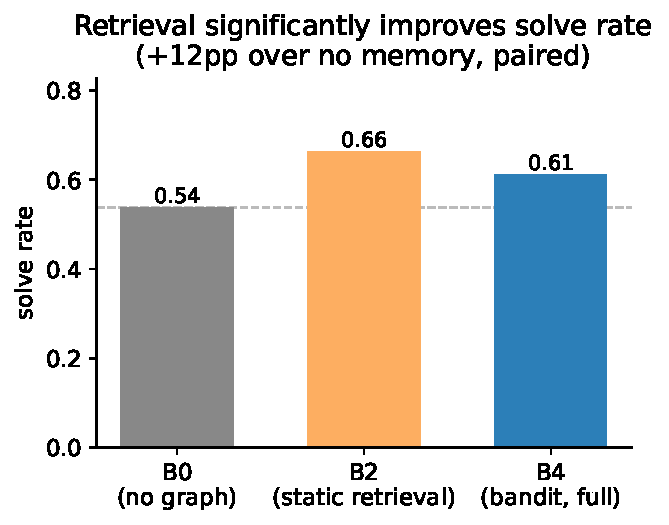
\includegraphics[width=0.86\linewidth]{fig_solve_rates.pdf}
\caption{No memory (B0) vs.\ static retrieval (B2) vs.\ the frozen bandit (B4).
Retrieval lifts solve rate; the bandit (B4) does \emph{not} improve on static
retrieval at this scale---its interest is in \emph{what it learns about lessons}.}
\label{fig:solve}
\end{figure}

\begin{figure}[t]\centering
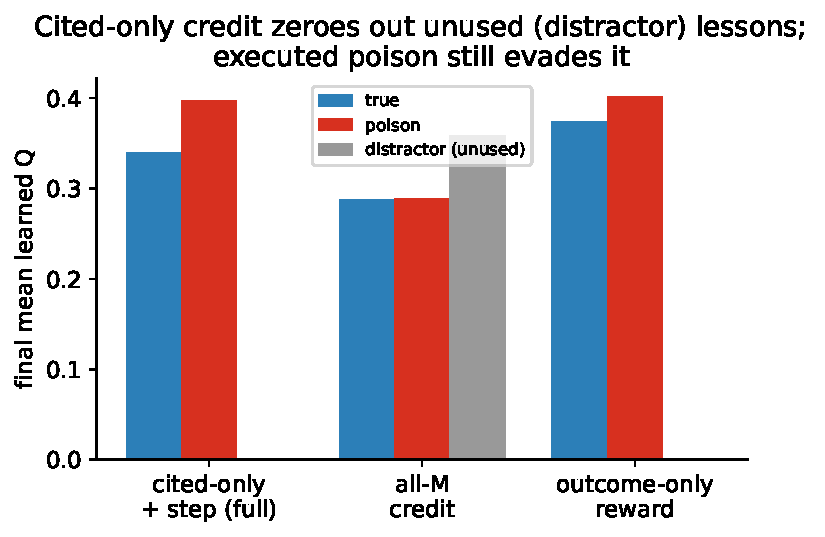
\includegraphics[width=0.96\linewidth]{fig_q_by_config.pdf}
\caption{Final learned value by ground-truth lesson type. Cited-only credit holds
\emph{unused} (distractor) lessons at zero; all-$M$ credit rewards them. But
\emph{executed} poison keeps a value indistinguishable from true lessons under every
configuration ($n{=}4$/label)---outcome credit cannot tell them apart.}
\label{fig:qcfg}
\end{figure}

\paragraph{(3) Executed poison evades the verifiable signal.}
When the false lesson is itself executed, cited-only credit cannot help. Poison
lessons name a wrong tool the agent runs (cited on \PoisonCite{} of the runs they
are sampled in); on a \emph{recovered} success they receive the same positive
credit as a useful lesson. The bandit therefore values poison
indistinguishably from true lessons ($Q_{\text{poison}}\eqd\Qpoison{}$, in this pilot
corpus numerically above $Q_{\text{true}}\eqd\Qtrue{}$; Fig.~\ref{fig:qtraj}), and the frozen bandit
does not beat static retrieval (\BfourSolve{}). The step-count lever does not
change this ($Q_{\text{poison}}\eqd\QpoisonOutcome{}$ under outcome-only reward as
well)---but for a reason that is itself a limitation: this corpus's poison misleads
via the \emph{wrong tool}, not a longer route, so the latent-poison mode the
step-count reward targets is never instantiated here, and that lever is
\emph{specified but not empirically tested} (\S\ref{sec:disc}). The clean statement
is: a verifiable success credits whichever tool was run, true or false; the
verifiable signal alone, even with action-grounded credit, does not attribute cause.

\begin{figure}[t]\centering
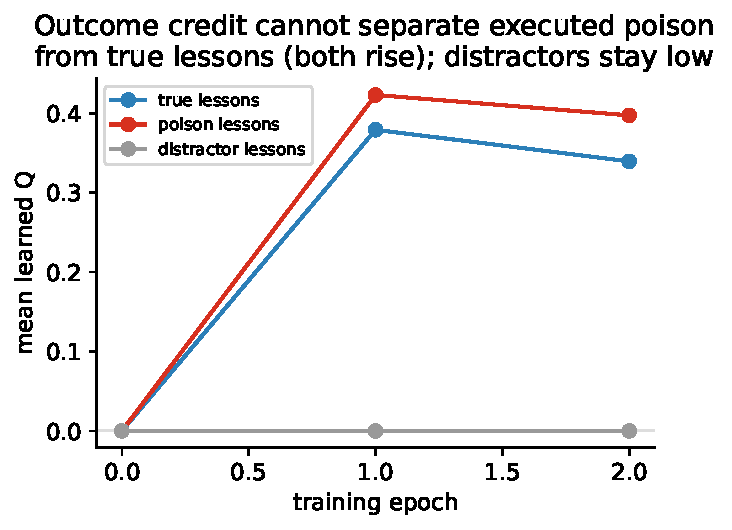
\includegraphics[width=0.86\linewidth]{fig_q_trajectory.pdf}
\caption{Learned value over training (full method). Executed poison tracks true
lessons---outcome credit cannot separate them---while unused distractors stay at
zero.}
\label{fig:qtraj}
\end{figure}

\paragraph{(4) An oracle-free causal probe measures marginal necessity.}
The leave-one-out re-rollout probe re-solves a challenge with and without a single
lesson, from a shared state, using only the flag. It measures single-lesson
\emph{necessity}; whether it can \emph{rank} the small per-item harm of a benign-false
lesson is a separate question that the lab-scale battery answers in the negative
(\S\ref{sec:results2}). On the ten probed
challenges---one true and one poison lesson each, twenty challenge--lesson pairs
(drawn from \emph{five} of the ten families: Base64, hex,
ROT13, reverse, gzip---the python-scripted families XOR and Caesar, and the
largest lift driver Base64$\circ$ROT13, are \emph{not} probed)---poison lessons
have marginal contribution
$\Delta\text{solve}\eqd\LooPoison{}$, while true lessons have $\eqd\LooTrue{}$.
That mean is bimodal: true lessons are causally \emph{necessary}
($\Delta\text{solve}\eqd{+}1.0$) only on the families the model cannot solve
unaided (ROT13, reverse) and $0$ where it already succeeds---so the probe measures
genuine necessity, not correlation with success. Two caveats are essential and we
state them plainly. First, the probe and the bandit $Q$ are different estimands
(single-lesson necessity vs.\ average reward over an $M{=}8$ context), so part of
the apparent ``probe succeeds where $Q$ fails'' gap is the change of estimand;
second, because our poison is a non-reaching wrong tool, its non-causality is
\emph{partly true by construction}---the stronger test has two halves: poison that
reaches the flag by a longer route, which we construct in Appendix~\ref{app:latent} and
probe against the \emph{step} channel only (the LOO probe was not run against it), and
LOO at matched $M{=}8$ conditioning, which remains future work.
The two remaining levers behave \emph{as specified}: gated write-back leaves
\GatedProvPct{} of new lessons (\GatedProv{}/\GatedTotal{}) provisional and trusts only
\GatedTrust{}/\GatedTotal{}, against \UngatedTrust{}/\UngatedTotal{}
(\UngatedTrustPct{}) trusted under ungating---though we report the provisional/trusted
split, not whether the trusted nodes were causally correct. Finally, off-policy evaluation recovers the logging policy's measured
value (doubly-robust \OpeDR{} vs.\ measured \OpeMeasured{}); this sanity check is
exact because the importance weights are unity when $\pi'\!=\!\pi_{\log}$, so it
\emph{validates the estimator} rather than identifying a better policy---the top
counterfactual temperature ($\tau\eqd\OpeBestTau{}$) lies within the logging
policy's CI (Fig.~\ref{fig:ope}). Validating under genuine distribution shift
requires a second on-GPU batch and is future work.

\begin{figure}[t]\centering
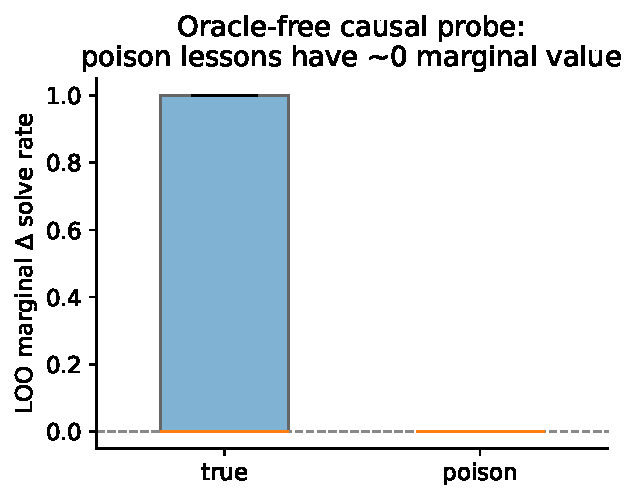
\includegraphics[width=0.74\linewidth]{fig_loo.pdf}
\caption{Leave-one-out marginal contribution, by ground-truth lesson type, on the
five LOO-probed families. Poison shows $\Delta\!\approx\!0$ here---partly true by
construction (a non-reaching wrong tool), and its small \emph{per-item} effect is not
rankable at scale (\S\ref{sec:results2})---where the bandit's outcome-credit had valued
it like a true lesson; true lessons are causal only where the model cannot already solve
unaided.}
\label{fig:loo}
\end{figure}

\begin{figure}[t]\centering
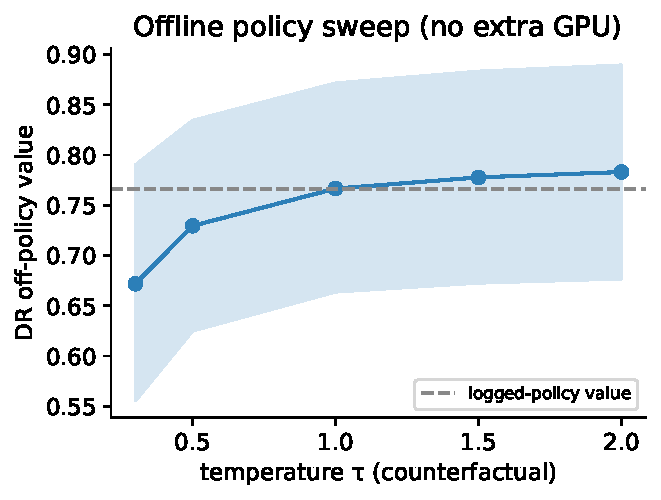
\includegraphics[width=0.82\linewidth]{fig_ope_sweep.pdf}
\caption{Off-policy value of counterfactual sampling temperatures from logged
propensities. The doubly-robust estimate recovers the logging policy's measured
value (dashed); the top candidate is within its CI, so the sweep validates the
estimator without identifying a significantly better policy at this $n$.}
\label{fig:ope}
\end{figure}

\paragraph{Summary.} The verifiable flag, with action-grounded credit, cheaply
removes value from \emph{unused} false lessons and (with gating) withholds trust
from \emph{premature} ones, but \emph{cannot} down-weight executed false lessons
the agent recovers from---the engineered bandit therefore does not improve on
static retrieval here. A causal re-rollout measures single-lesson necessity on the
subset we probe---and \S\ref{sec:results2} pushes this to its limit, showing that even
this gold standard cannot rank the per-item harm of a benign-false lesson. This maps
which false-lesson modes the verifiable signal alone can contain, and where causal credit
reaches and where it does not.